%%%%%%%%%%%%%%%%%%%%%%%%%%%%%%%%%%%%%
%                                   %
% Compile with XeLaTeX              %
%                                   %
% Questions or comments:            %
%                                   %
% joshua dot mcneill at uga dot edu %
%                                   %
%%%%%%%%%%%%%%%%%%%%%%%%%%%%%%%%%%%%%

\documentclass{beamer}
  % Read in standard preamble (cosmetic stuff)
  %%%%%%%%%%%%%%%%%%%%%%%%%%%%%%%%%%%%%%%%%%%%%%%%%%%%%%%%%%%%%%%%
% This is a standard preamble used in for all slide documents. %
% It basically contains cosmetic settings.                     %
%                                                              %
% Joshua McNeill                                               %
% joshua dot mcneill at uga dot edu                            %
%%%%%%%%%%%%%%%%%%%%%%%%%%%%%%%%%%%%%%%%%%%%%%%%%%%%%%%%%%%%%%%%

% Beamer settings
% \usetheme{Berkeley}
\usetheme{CambridgeUS}
% \usecolortheme{dove}
% \usecolortheme{rose}
\usecolortheme{seagull}
\usefonttheme{professionalfonts}
\usefonttheme{serif}
\setbeamertemplate{bibliography item}{}

% Packages and settings
\usepackage{fontspec}
  \setmainfont{Charis SIL}
\usepackage{hyperref}
  \hypersetup{colorlinks=true,
              allcolors=blue}
\usepackage{graphicx}
  \graphicspath{{../../figures/}}
\usepackage[normalem]{ulem}
\usepackage{enumerate}

% Document information
\author{M. McNeill}
\title[FREN2001]{Français 2001}
\institute{\url{joshua.mcneill@uga.edu}}
\date{}

%% Custom commands
% Lexical items
\newcommand{\lexi}[1]{\textit{#1}}
% Gloss
\newcommand{\gloss}[1]{`#1'}
\newcommand{\tinygloss}[1]{{\tiny`#1'}}
% Orthographic representations
\newcommand{\orth}[1]{$\langle$#1$\rangle$}
% Utterances (pragmatics)
\newcommand{\uttr}[1]{`#1'}
% Sentences (pragmatics)
\newcommand{\sent}[1]{\textit{#1}}
% Base dir for definitions
\newcommand{\defs}{../definitions}


  % Packages and settings
  \usepackage[linguistics]{forest}
  \usepackage{adjustbox}

  % Document information
  \subtitle[Phonetics Intro]{Introduction to Phonetics}

  %% Custom commands
  % Subsection/frame titles
  \newcommand{\suboneone}{Definition}
  \newcommand{\subtwoone}{How we study sounds}
  \newcommand{\subtwotwo}{Why a new alphabet}
  \newcommand{\subtwothree}{Organizing sounds}
  \newcommand{\subtwofour}{The charts}

\begin{document}
  % Read in the standard intro slides (title page and table of contents)
  %%%%%%%%%%%%%%%%%%%%%%%%%%%%%%%%%%%%%%%%%%%%%%%%%%%%%%%%%%%%%%%%
% This is a standard set of intro slides used in for all slide %
% documents. It basically contains the title page and table of %
% contents.                                                    %
%                                                              %
% Joshua McNeill                                               %
% joshua dot mcneill at uga dot edu                            %
%%%%%%%%%%%%%%%%%%%%%%%%%%%%%%%%%%%%%%%%%%%%%%%%%%%%%%%%%%%%%%%%

\begin{frame}
  \titlepage
  \tiny{Office: % Basically a variable for office hours location
Gilbert 121\\
        Office hours: % Basically a variable for office hours
 lundi, mercredi, vendredi 10:10--11:10
}
\end{frame}

\begin{frame}
  \tableofcontents[hideallsubsections]
\end{frame}

\AtBeginSection[]{
  \begin{frame}
    \tableofcontents[currentsection,
                     hideallsubsections]
  \end{frame}
}


  \section{What is phonetics?}
    \subsection{\suboneone}
      \begin{frame}{\suboneone}
        \only<1-3>{
          \begin{block}<1-3>{}
            % Phonetics
The study of the minimal units that make up a language
 (i.e., words, consonants, vowels, intonation, and stress)
          \end{block}
          \begin{block}<2-3>{}
            The three broad areas of phonetics:
            \begin{itemize}
              \item \alert<3>{Articulatory phonetics}
                \begin{itemize}
                  \item % Articulatory phonetics
The study of the physiological production of speech sounds

                \end{itemize}
              \item \alert<3>{Acoustic phonetics}
                \begin{itemize}
                  \item % Acoustic phonetics
The study of the acoustic properties of speech sounds and their transmission

                \end{itemize}
              \item Auditory phonetics
                \begin{itemize}
                  \item % Auditory phonetics
The study of the perception of speech sounds

                \end{itemize}
            \end{itemize}
          \end{block}
        }
        % \only<4>{
        %   \begin{alertblock}{}
        %     This is an aspect of \emph{your} language (i.e., your personal mental lexicon and mental grammar)
        %   \end{alertblock}
        % }
      \end{frame}

  \section{Representing speech sounds}
    \subsection{\subtwoone}
      \begin{frame}{\subtwoone}
        \only<1-2>{
          \begin{columns}
            \column{0.48\linewidth}
              \begin{block}{Articulatory phonetics}
                Several tools are used:
                \begin{itemize}
                  \item \href{https://www.youtube.com/watch?v=DcNMCB-Gsn8}{X-ray}
                  \item Ultrasound
                  \item Palatography
                    \begin{itemize}
                      \item Dye is added to the tongue and roof of the mouth and a picture is taken after pronouncing a sound
                    \end{itemize}
                \end{itemize}
              \end{block}
            \column{0.48\linewidth}
              \uncover<2->{
                % \begin{center}
                  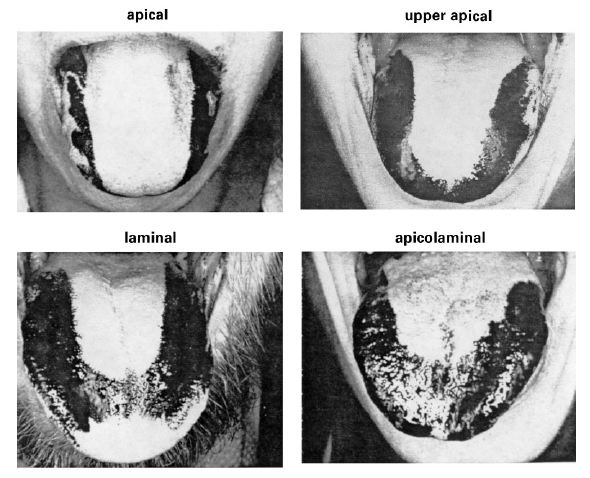
\includegraphics[scale=0.225]{palatography.jpg}
                % \end{center}
              }
          \end{columns}
        }
        \only<3>{
          \begin{block}{Acoustic phonetics}
            \begin{itemize}
              \item Spectrograms
            \end{itemize}
            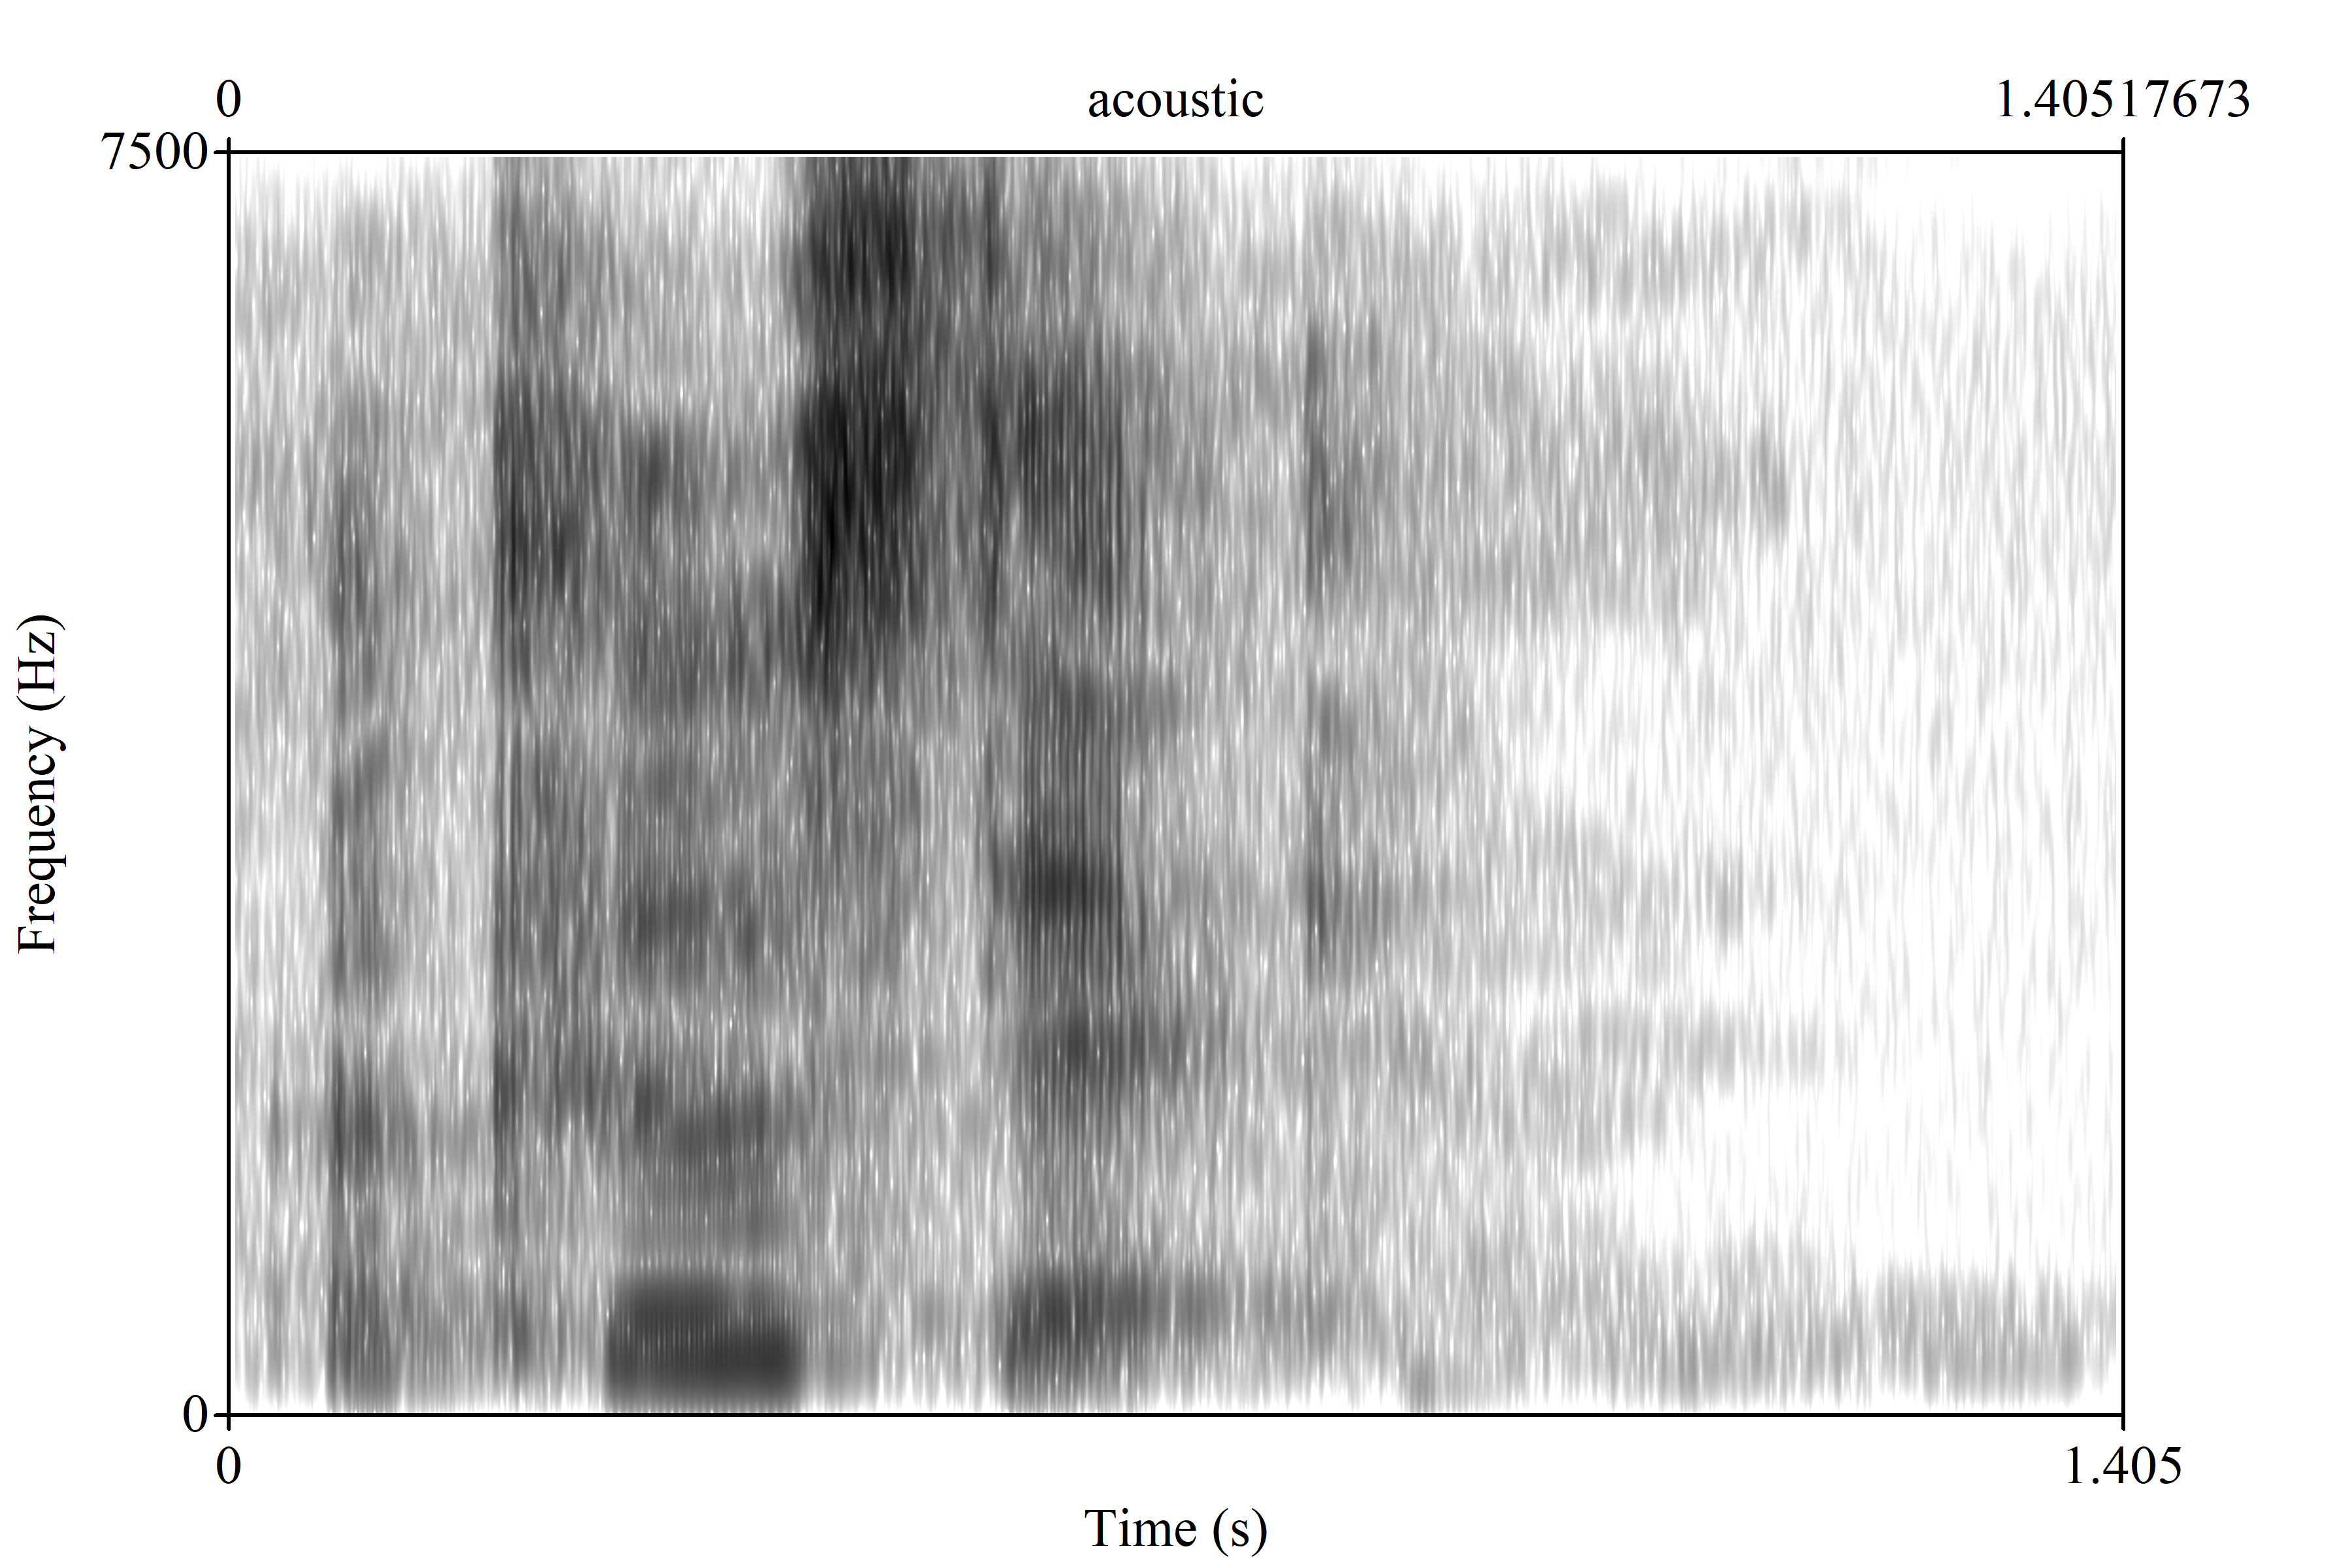
\includegraphics[scale=0.55]{sharcoustic.jpg}
          \end{block}
        }
        \only<4-7>{
          \begin{block}{Impressionistic transcription}
            \href{https://youtu.be/J2oEmPP5dTM?t=51}{Satchmo and tomatoes}
            \begin{itemize}
              \item<5-> təˈmeɪ.ɾoʊ
              \item<5-> təˈmɑ.ɾoʊ
              \item<6-> təˈmeɪ.ɾə
            \end{itemize}
          \end{block}
          \begin{alertblock}<7->{International phonetic alphabet (IPA)}
            % Read in the definition of the IPA
            % The international phonetic alphabet (IPA)
A \emph{language independent} alphabet for which there is a \emph{one-to-one} correspondence between sounds and symbols

          \end{alertblock}
        }
      \end{frame}

    \subsection{\subtwotwo}
      \begin{frame}{\subtwotwo}
        \begin{block}{English orthography is not exact enough}
          \begin{itemize}
            \item Multiple representations for individual sounds
            \begin{itemize}
              \item Why not \orth{tomatoe} like \orth{toe}?
            \end{itemize}
            \item Multiple individual sounds from one representation
            \begin{itemize}
              \item The two \orth{t}s in \orth{tomato} represent [t] and [ɾ]
            \end{itemize}
            \item One letter can represent multiple sounds
            \begin{itemize}
              \item The \orth{x} in \orth{exit} represents [ks]
            \end{itemize}
            \item There are silent letters
            \begin{itemize}
              \item The \orth{e} in \orth{toe} is silent
            \end{itemize}
          \end{itemize}
        \end{block}
      \end{frame}

    \subsection{\subtwothree}
      \begin{frame}[t]{\subtwothree}
        \begin{block}{Smallest to biggest}
          segments $\rightarrow$ syllables $\rightarrow$ suprasegmentals
        \end{block}
        \only<2-3>{
          \begin{alertblock}{A segment}
            % Read in the definition of a segment
            % Segment
A consonant or a vowel

            \begin{itemize}
              \item<3> \alert{Consonant}: % Consonant
A segment produced by restricting airflow in the vocal tract

              \item<3> \alert{Vowel}: % Vowel
A segment that is produced without restricting airflow in the vocal tract

            \end{itemize}
          \end{alertblock}
        }
        \only<4>{
          \begin{block}{The phthongs}
            \begin{itemize}
              \item A \alert{monophthong}: % Monophthong
Only one vowel in a syllable

              \item A \alert{diphthong}: % Diphthong
More than one vowel in a syllable

            \end{itemize}
          \end{block}
        }
        \only<5-6>{
          \begin{columns}
            \column{0.5\textwidth}
              \only<5>{
                \begin{alertblock}{A syllable}
                  % Read in the definition of a syllable
                  % Syllable
A unit of speech made up of one or more adjacent vowels, optionally surrounded by consonants

                \end{alertblock}
              }
              \only<6>{
                \begin{alertblock}{A nucleus}
                  % Read in the definition of a nucleus
                  % Nucleus
The required vocalic part of a syllable

                \end{alertblock}
              }
            \column{0.5\textwidth}
              \only<5>{
                % Read in a tree graph of a syllable
                % This uses the forest package to print a basic syllable structure
\begin{forest}
  [ Syllable
    [ Onset
      [ p, tier=segment ]
    ]
    [ Rhyme
      [ Nucleus
        [ ɪ, tier=segment ]
      ]
      [ Coda
        [ n, tier=segment ]
      ]
    ]
  ]
\end{forest}

              }
              \only<6>{
                \begin{forest}
                  [ Syllable
                    [ Onset
                      [ p, tier=segment ]
                    ]
                    [ \alert{Rhyme}
                      [ \alert{Nucleus}
                        [ \alert{ɪ}, tier=segment ]
                      ]
                      [ Coda
                        [ n, tier=segment ]
                      ]
                    ]
                  ]
                \end{forest}
              }
          \end{columns}
        }
        \only<7>{
          \begin{alertblock}{A suprasegmental}
            % Read in definition of a suprasegmental
            % Suprasegmental
A sound feature that applies to a whole syllable and is best understood in relation to how it changes across syllables

            \begin{itemize}
              \item Stress, intonation, tone, etc.
            \end{itemize}
          \end{alertblock}
        }
      \end{frame}

    \subsection{\subtwofour}
      \begin{frame}[t]{\subtwofour}
        \begin{block}<1-2>{The sounds of English}
          \only<1>{Consonants}
          \only<2>{Vowels}
        \end{block}
        \only<1>{
          \begin{adjustbox}{width=\textwidth}
            % Read in English IPA consonant chart
            %%%%%%%%%%%%%%%%%%%%%%%%%%%%%%%%%%%%%%%%%%%%%%%%%%%%%%%%%%
% This creates an English IPA chart for consonants       %
%                                                        %
% Compiled from material_IPA_en_chart.tex when a         %
% standalone document is needed                          %
%                                                        %
% -Joshua McNeill (joshua dot mcneill at uga dot edu)    %
%%%%%%%%%%%%%%%%%%%%%%%%%%%%%%%%%%%%%%%%%%%%%%%%%%%%%%%%%%

\begin{tabular}{| l | c c | c c | c c | c c | c c | c c | c c | c c | c c | c c | c c |}
  \hline
  & \multicolumn{2}{c}{Bilabial} & \multicolumn{2}{c}{Labiodental} & \multicolumn{2}{c}{Dental} & \multicolumn{2}{c}{Alveolar} & \multicolumn{2}{c}{Postalveolar} & \multicolumn{2}{c}{Retroflex} & \multicolumn{2}{c}{Palatal} & \multicolumn{2}{c}{Velar} & \multicolumn{2}{c}{Uvular} & \multicolumn{2}{c}{Pharyngeal} & \multicolumn{2}{c}{Glottal} \\
  \hline
  Plosive/Stop & p & b &   &   &   &   & t & d &   &   & & & &   & k & ɡ & & & & & ʔ & \\
  \hline
  Nasal        &   & m &   &   &   &   &   & n &   &   & & & &   &   & ŋ & & & & &   & \\
  \hline
  Trill        &   &   &   &   &   &   &   &   &   &   & & & &   &   &   & & & & &   & \\
  \hline
  Tap/Flap     &   &   &   &   &   &   &   & ɾ &   &   & & & &   &   &   & & & & &   & \\
  \hline
  Fricative    &   &   & f & v & θ & ð & s & z & ʃ & ʒ & & & &   &   &   & & & & & h & \\
  \hline
  \begin{tabular}{@{} l @{}}
    Lateral \\
    fricative
  \end{tabular}&   &   &   &   &   &   &   &   &   &   & & & &   &   &   & & & & &   & \\
  \hline
  Approximant  &   &   &   &   &   &   &   & ɹ &   &   & & & & j &   &   & & & & &   & \\
  \hline
  \begin{tabular}{@{} l @{}}
    Lateral\\
    approximant
  \end{tabular}&   &   &   &   &   &   &   & l &   &   & & & &   &   &   & & & & &   & \\
  \hline
\end{tabular}

          \end{adjustbox}
        }
        \only<2>{
          \begin{adjustbox}{height=4.5cm}
            % Read in English IPA vowel chart
            %%%%%%%%%%%%%%%%%%%%%%%%%%%%%%%%%%%%%%%%%%%%%%%%%%%%%%%%%%%%%%%%%%%%%%%%%%%%%%%%%%%%%
% This creates an English IPA chart for vowels                                      %
%                                                                                   %
% Compiled from material_IPA_en_chart.tex when a                                    %
% standalone document is needed                                                     %
%                                                                                   %
% Code is only slightly modified from:                                              %
%   https://tex.stackexchange.com/questions/156955/tikz-pgf-linguistics-vowel-chart %
%                                                                                   %
% -Joshua McNeill (joshua dot mcneill at uga dot edu)                               %
%%%%%%%%%%%%%%%%%%%%%%%%%%%%%%%%%%%%%%%%%%%%%%%%%%%%%%%%%%%%%%%%%%%%%%%%%%%%%%%%%%%%%

% Custom command
\def\V(#1,#2){barycentric cs:hf={(3-#1)*(2-#2)},hb={(3-#1)*#2},lf={#1*(2-#2)},lb={#1*#2}}

% Chart
\begin{tikzpicture}[scale=3]
  \large
  \tikzset{
    vowel/.style={fill=white, anchor=mid, text depth=0ex, text height=1ex},
    dot/.style={circle,fill=black,minimum size=0.4ex,inner sep=0pt,outer sep=-1pt},
  }
  \coordinate (hf) at (0,2); % high front
  \coordinate (hb) at (2,2); % high back
  \coordinate (lf) at (1,0); % low front
  \coordinate (lb) at (2,0); % low back
  \def\V(#1,#2){barycentric cs:hf={(3-#1)*(2-#2)},hb={(3-#1)*#2},lf={#1*(2-#2)},lb={#1*#2}}

  % Draw the horizontal lines first.
  \draw (\V(0,0)) -- (\V(0,2));
  \draw (\V(1,0)) -- (\V(1,2));
  \draw (\V(2,0)) -- (\V(2,2));
  \draw (\V(3,0)) -- (\V(3,2));

  % Place all the unrounded-rounded pairs next, on top of the horizontal lines.
  \path (\V(0,0))     node[vowel, left] {i}          node[vowel, right] { }          node[dot] {};
  \path (\V(0,1))     node[vowel, left] { }          node[vowel, right] { }          node[dot] {};
  \path (\V(0,2))     node[vowel, left] { }          node[vowel, right] {u}          node[dot] {};
  \path (\V(0.5,0.4)) node[vowel, left] {\textbf{ɪ}} node[vowel, right] { }          node[   ] {};
  \path (\V(0.5,1.6)) node[vowel, left] { }          node[vowel, right] {\textbf{ʊ}} node[   ] {};
  \path (\V(1,0))     node[vowel, left] {e}          node[vowel, right] { }          node[dot] {};
  \path (\V(1,1))     node[vowel, left] { }          node[vowel, right] { }          node[dot] {};
  \path (\V(1,2))     node[vowel, left] { }          node[vowel, right] {o}          node[dot] {};
  \path (\V(2,0))     node[vowel, left] {\textbf{ɛ}} node[vowel, right] { }          node[dot] {};
  \path (\V(2,1))     node[vowel, left] { }          node[vowel, right] { }          node[dot] {};
  \path (\V(2,2))     node[vowel, left] {\textbf{ʌ}} node[vowel, right] {ɔ}          node[dot] {};
  \path (\V(2.5,0))   node[vowel, left] {\textbf{æ}} node[vowel, right] { }          node[   ] {};
  \path (\V(3,0))     node[vowel, left] {a}          node[vowel, right] { }          node[dot] {};
  \path (\V(3,2))     node[vowel, left] {ɑ}          node[vowel, right] { }          node[dot] {};

  % Draw the vertical lines.
  \draw (\V(0,0)) -- (\V(3,0));
  \draw (\V(0,1)) -- (\V(3,1));
  \draw (\V(0,2)) -- (\V(3,2));

  % Place the unpaired symbols last, on top of the vertical lines.
  \path (\V(1.5,1))   node[vowel]       {\textbf{ə}};
  \path (\V(-0.25,0)) node[vowel]       {front};
  \path (\V(-0.25,1)) node[vowel]       {central};
  \path (\V(-0.25,2)) node[vowel]       {back};
  \path (\V(0,-0.5))  node[vowel]       {high};
  \path (\V(1,-0.8))  node[vowel]       {high-mid};
  \path (\V(2,-1.55)) node[vowel]       {low-mid};
  \path (\V(3,-2.95)) node[vowel]       {low};
\end{tikzpicture}

          \end{adjustbox}
        }
        \only<3>{
          \begin{block}{Resources}
            % A set of links to useful resources when dealing articulatory phonetics
\begin{itemize}
  \item To hear these sounds: \url{http://web.uvic.ca/ling/resources/ipa/charts/IPAlab/IPAlab.htm} and \url{https://americanipachart.com/}
  \item To type these symbols: \url{https://ipa.typeit.org/}
\end{itemize}

          \end{block}
        }
      \end{frame}
\end{document}
